\documentclass{scrreprt}
\usepackage{listings}
\usepackage{underscore}
\usepackage{graphicx}
\usepackage[bookmarks=true]{hyperref}
\usepackage[utf8]{inputenc}
\usepackage[spanish]{babel}
\usepackage{tabularx}

\hypersetup{
    bookmarks=false,    % show bookmarks bar?
    pdftitle={Documento de Arquitectura de Software},    % title
    pdfauthor={Albany Armenta},                     % author
    pdfsubject={TeX and LaTeX},                        % subject of the document
    pdfkeywords={TeX, LaTeX, graphics, images}, % list of keywords
    colorlinks=true,       % false: boxed links; true: colored links
    linkcolor=blue,       % color of internal links
    citecolor=black,       % color of links to bibliography
    filecolor=black,        % color of file links
    urlcolor=purple,        % color of external links
    linktoc=page            % only page is linked
}%
\def\myversion{1.0 }
\date{}
%\title
\usepackage{hyperref}
\begin{document}

\begin{flushright}
    \rule{16cm}{5pt}\vskip1cm
    \begin{bfseries}
        \Huge{Documento de Arquitectura de Software}\\
        \vspace{1.5cm}
        \textbf{Sistema para la Recolección, Procesamiento y Clasificación a partir de Wi-Fi CSI}\\
        \vspace{1.5cm}
        \LARGE{Versión \myversion}\\
        \vspace{1.5cm}
        Elaborado por: Jesús A. Armenta-García\\
        \vspace{1.5cm}
        \today\\
    \end{bfseries}
\end{flushright}

\tableofcontents

\chapter{Introducción}

\section{Propósito}
El propósito de este documento es presentar el sistema \emph{Herramienta de Recolección, Procesamiento y Clasificación a partir de Wi-Fi CSI} y describir su arquitectura interna desde diferentes perspectivas del desarrollo de software, proporcionando una descripción detallada de las funcionalidades del sistema y las interacciones entre cada uno de los componentes internos. Esto con la finalidad de facilitar las tareas de mantenimiento o extensión de funcionalidades del sistema. 

\section{Audiencia Objetivo}
Este documento esta dirigido a desarrolladores de software, administradores de proyecto y usuarios interesados en el funcionamiento del sistema que aquí se presenta. 

\section{Alcance del Proyecto}
Para el desarrollo del sistema \emph{Herramienta de Recolección, Procesamiento y Clasificación a partir de Wi-Fi CSI} se planteó un proyecto con duración de cuatro años el cual abarcaba actividades de investigación, desarrollo, pruebas, divulgación y difusión, culminando con la difusión del sistema ante la comunidad científica para promover su utilización e impulsar el desarrollo de sistemas de monitoreo con base en señales Wi-Fi, difundiendo un caso de uso del sistema para la identificación de actividades humanas y monitoreo de frecuencia respiratoria. 

Cabe destacar que lo que se presenta en este documento corresponde al segundo de los cuatro años definidos para el proyecto, en donde las actividades se enfocaban en el proceso de desarrollo y pruebas del sistema. Por lo tanto el alcance de este documento es llegar a ofrecer, como se mencionó anteriormente, una descripción detallada de las funcionalidades del sistema y las interacciones entre los componentes internos a partir de las siguientes vistas: 
\begin{itemize}
    \item \textbf{Vista de Casos de Uso:}
    \item \textbf{Vista Lógica: }
    \item \textbf{Vista de Procesos: }
    \item \textbf{Vista de Implementación: }
    \item \textbf{Vista de Despliegue: }
\end{itemize}

\chapter{Descripción del Sistema}

\section{Descripción General}
"IICT WEBSITE" is the replacement of the manual hard copy result process. The data have been stored in the hard file or papers, this website will store all of those in the website. Main goal of this project is to minimize the work and maximize the result of this result processing system.

\section{Procesos del Sistema }
El sistema se divide en cinco procesos (\emph{tasks}, de acuerdo a FreeRTOS), Main Task, Wi-Fi Task, Processor Task, CSI Task y Predictor Task. 
\begin{itemize}
  \item \textbf{Main Task: }
  \item \textbf{Wi-Fi Task: }
  \item \textbf{Processor Task: }
  \item \textbf{CSI Task: }
  \item \textbf{Predictor Task: }
\end{itemize}

\section{Plataforma de Desarrollo e Implementación}
Descripcion de ESP IDF y ESP32

\chapter{Vista de Casos de Uso}

Los actores que intervienen en el sistema, en conjunto con la descripción de cada uno de ellos se presenta en el Cuadro \ref{tab:actores}. Por otra parte, las interacciones de cada uno de ellos con el sistema se ilustran en la Figura \ref{fig:casos_uso}
\begin{table}[h!]
    \caption{Descripción de Actores en el Sistema}
    \begin{tabularx}{\textwidth}{|l | X |}
        \hline
        \textbf{Actor} & \textbf{Descripción} \\
        \hline 
        Administrador & El Investigador es el responsable de realizar la configuración de la etapa de recolección del sistema, teniendo que definir la direcciones MAC del dispositivo receptor y transmisor para establecer el enlace de comunicación entre ambos. \\
        \hline 
        Persona a Monitorear & Corresponde a la persona a la cual se desea monitorear por medio del sistema. Si bien este actor no ejerce de manera directa una interacción con el sistema, sus acciones son capturadas por el sistema. \\ 
        \hline 
    \end{tabularx}
    \label{tab:actores}
\end{table}

\begin{figure}[h!]
    \centering
    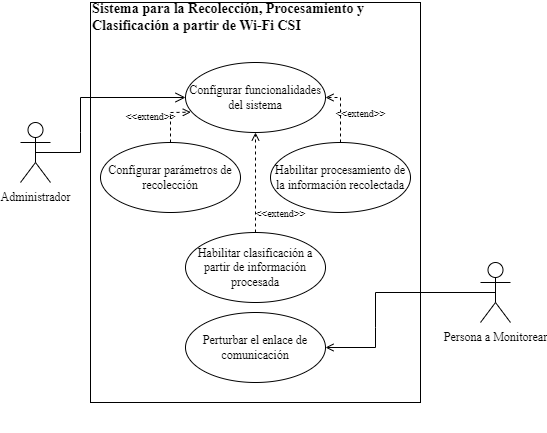
\includegraphics[scale = 0.57]{images/casos_uso.png}
    \caption{Diagrama de Casos de Uso}
    \label{fig:casos_uso}
\end{figure}

\chapter{Vista Lógica}
Para describir el sistema desde una vista lógica se utiliza un \emph{Diagrama de Componentes} el cual se muestra en la Figura \ref{}. En este podemos observar que los proceso del sistema también pueden ser catalogados como componentes del mismo con funcionalidades específicas e interacciones marcadas entre sí. 


\chapter{Vista de Procesos}

\chapter{Vista de Implementación}

\chapter{Vista de Despliegue}



\end{document}